\subsection{1D exact}

\begin{frame}{1D: Encodings + Error Measure}
    \begin{minipage}{.6\textwidth}

        \begin{itemize}
            \item Relative error $\epsilon$
            \item Different encodings blocks
                  \begin{itemize}
                      \item A: small bond dimension
                      \item E: no spurious blocks
                      \item F: well conditioned
                  \end{itemize}
        \end{itemize}

    \end{minipage}
    \begin{minipage}{.39\textwidth}

        \begin{table}[]
            \caption*{$\chi$}
            \begin{tabular}{l l|l l }
                                                       &   & \multicolumn{2}{c}{Encoding}       \\
                                                       &   & A                            & E/F \\
                \hline
                \multirow{3}{*}{\rotatebox{90}{Order}} & 3 & 5                            & 10  \\
                                                       & 5 & 21                           & 42  \\
                                                       & 7 & 85                           & 170 \\
            \end{tabular}
        \end{table}
    \end{minipage}
\end{frame}

\begin{frame}{1D: Transverse Field Ising}

    \begin{figure}
        \center
        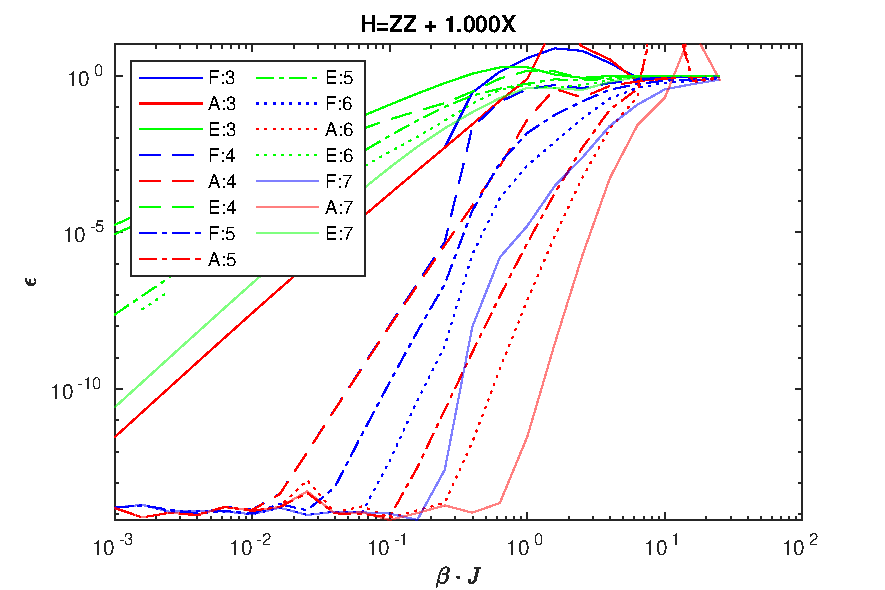
\includegraphics[height=\textheight]{../Figuren/benchmarking/t_ising.pdf}
    \end{figure}

\end{frame}

\begin{frame}{1D: Heisenberg XXX}

    \begin{figure}
        \center
        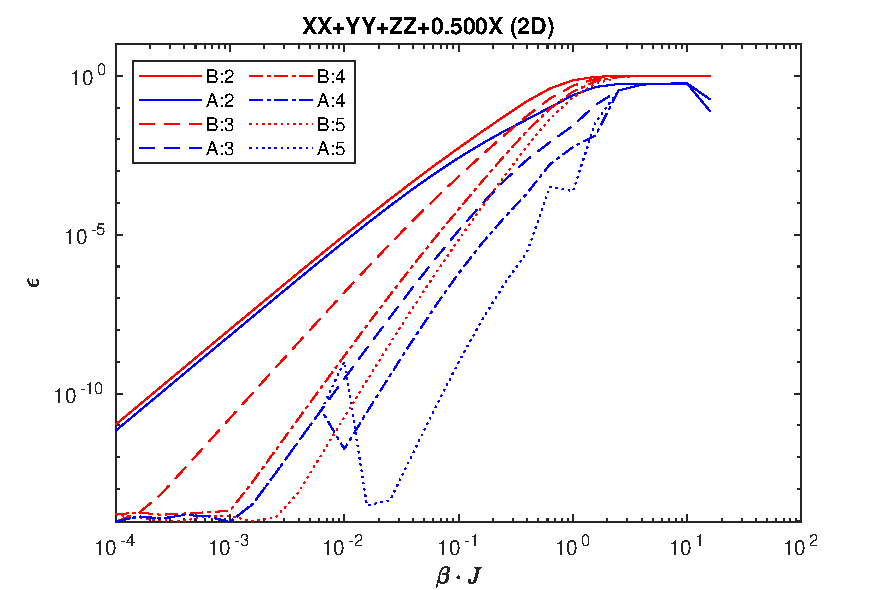
\includegraphics[height=\textheight]{../Figuren/benchmarking/t_heis_XXX.pdf}
    \end{figure}

\end{frame}

\subsection{2D exact}

\begin{frame}{2D: Encodings + Error Measure}

    \begin{minipage}{.6\textwidth}
        \begin{itemize}
            \item Relative error $\epsilon$ more challenging
            \item Encodings based on A (order 5)
                  \begin{itemize}
                      \item \makebox[2.07cm]{No loops\hfill}$\vcenter{\hbox{\pepob{5}{3}{{
                                                    "-","-", "-",     "-",
                                                    "","","","",
                                                    "","-","",""}}{{
                                                    "-","",
                                                    "-","",
                                                    "-","",
                                                    "-","",
                                                    "-",""}}{{
                                                    1,1,1,1,1,
                                                    1,0,0,0,0,
                                                    1,1,0,1,1}} }} $
                      \item \makebox[2cm]{+Plaquette\hfill}$\vcenter{\hbox{{\pepob{2}{2}{{
                                                            "","",}}{{
                                                            "","",}}{{
                                                            0,0,
                                                            0,0}}} }}$
                      \item \makebox[2cm]{+Extensions\hfill}$\vcenter{\hbox{\pepob{5}{3}{{
                                                    "-","-", "-","-",
                                                    "","","","",
                                                    "","","",""}}{{
                                                    "-","",
                                                    "-","",
                                                    "-","",
                                                    "-","",
                                                    "-",""}}{{
                                                    1,1,1,1,1,
                                                    1,1,0,0,0,
                                                    1,1,0,0,1}} }} $
                  \end{itemize}
        \end{itemize}

    \end{minipage}
    \begin{minipage}{.39\textwidth}
        \begin{table}[]
            \begin{tabular}{l|l }
                           & $\chi$ \\
                \hline              \\
                no loops   & 21     \\
                plaquette  & 27     \\
                extensions & 43     \\
            \end{tabular}
        \end{table}

    \end{minipage}

\end{frame}

\begin{frame}{2D: TFI}

    \begin{figure}
        \center
        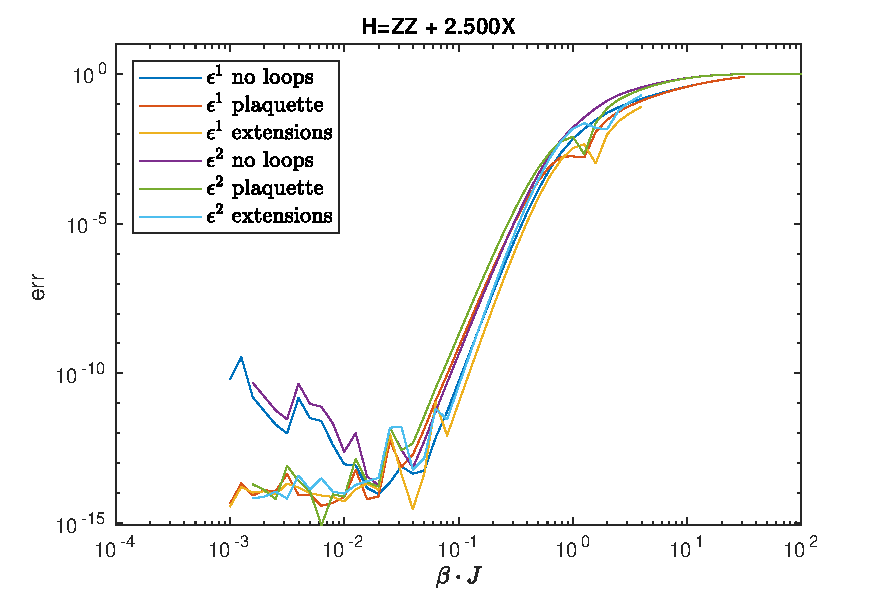
\includegraphics[height=\textheight]{../Figuren/benchmarking/2D_Err01_t_sing.pdf}
    \end{figure}

\end{frame}

\begin{frame}{Conclusion}
    \begin{itemize}
        \item Large $\beta$-steps
        \item Real time evolution
        \item Encoding
        \item Truncation $\chi$
    \end{itemize}
\end{frame}

\subsection{2D Transverse Ising model}

\begin{frame}{2D TFI: Introduction}
    \begin{minipage}{0.35\textwidth}
        \begin{itemize}
            \item Phase Transition
            \item Criticality
            \item Finite size scaling
                  \begin{itemize}
                      \item Observables:

                            $m$, $S$ and $\xi$
                      \item Parameters:

                            $T_c$, exponents
                  \end{itemize}
            \item $\Gamma=2.5$ and $\Gamma=0$
            \item VUMPS ($\chi$,$\delta^{-1}$)
        \end{itemize}
    \end{minipage}
    \begin{minipage}{0.64\textwidth}
        \begin{figure}
            \centering
            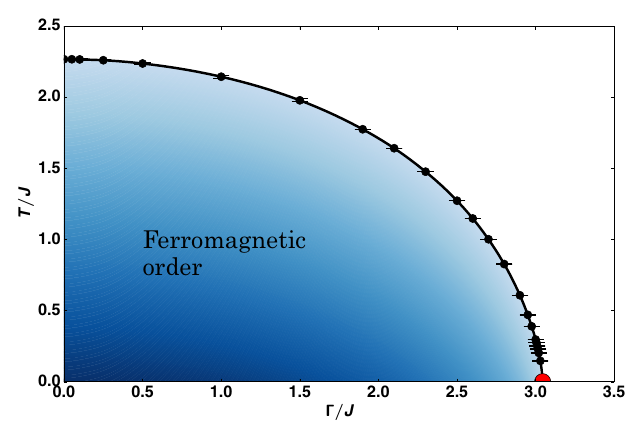
\includegraphics[width=\linewidth]{../Figuren/phsyics/2disingphase.png}
            \caption*{Figure taken from \cite{Hesselmann2016}  }
        \end{figure}
    \end{minipage}
\end{frame}

\begin{frame}{2D TFI: $\Gamma=2.5$}
    \begin{minipage}{.75\textwidth}
        \begin{figure}
            \center
            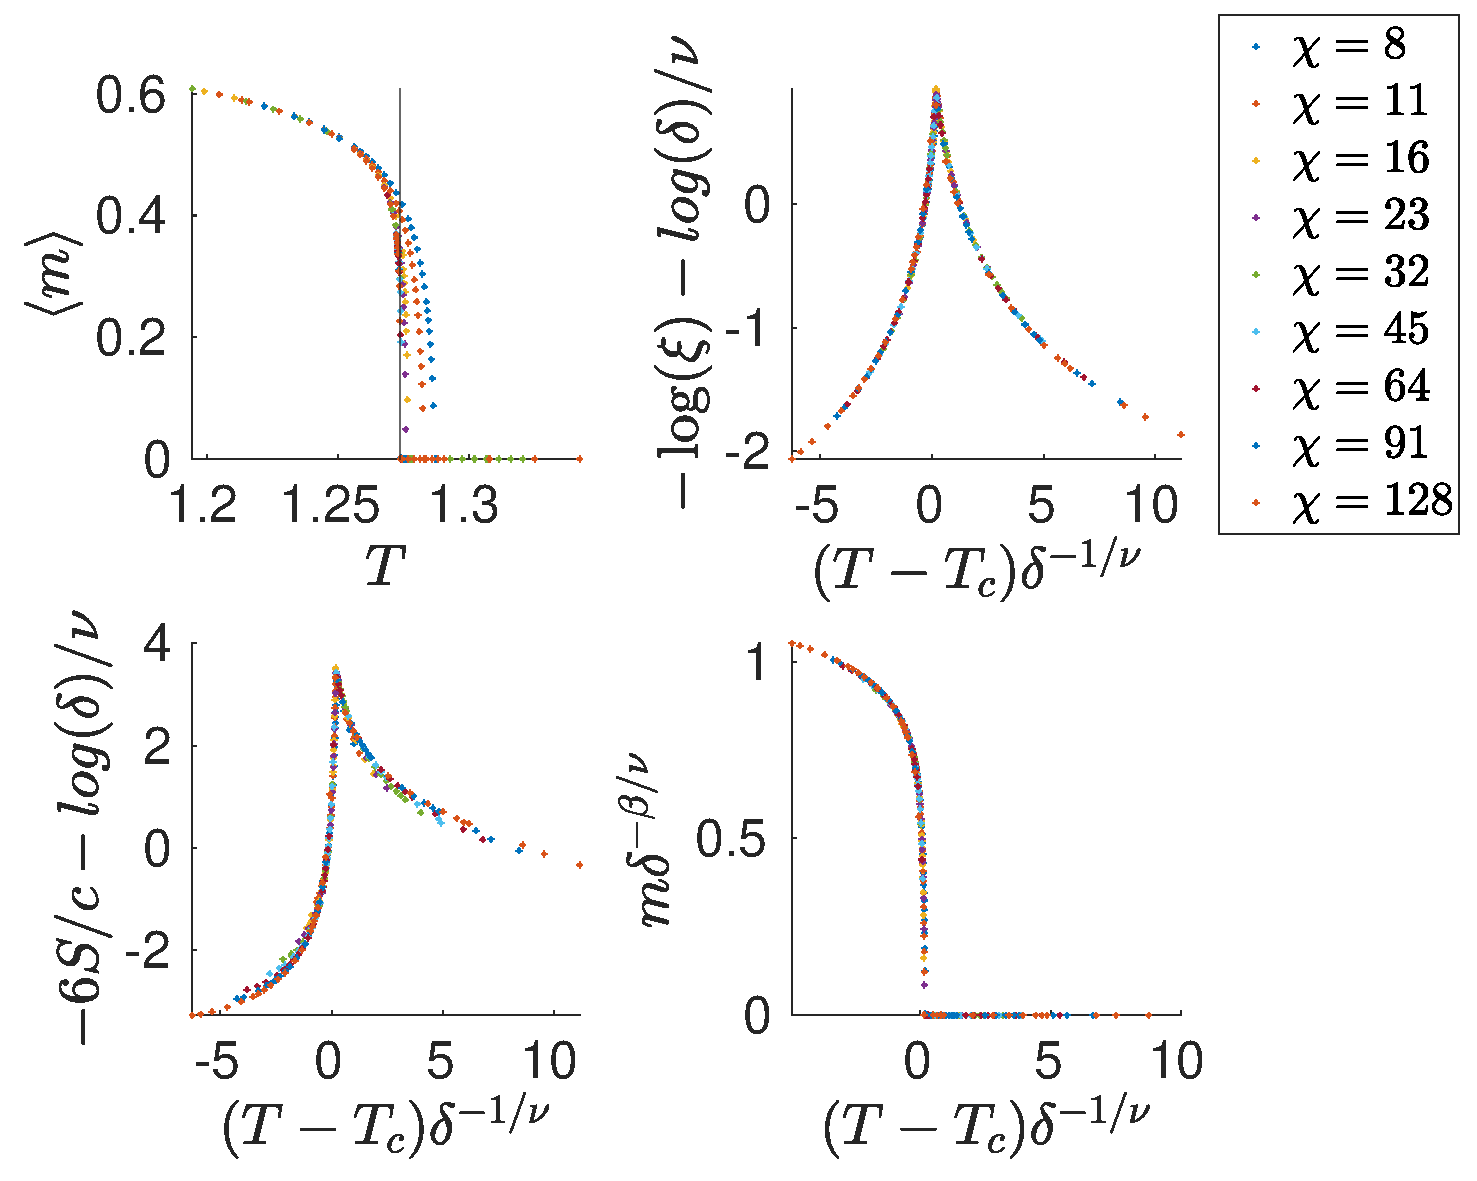
\includegraphics[height=\textheight]{../Figuren/phasediag/g25/zoomed_small.pdf}
        \end{figure}
    \end{minipage}
    \begin{minipage}{.24\textwidth}
        \begin{table}[]

            \begin{tabular}{l|l }
                    & $T_c$     \\
                \hline          \\
                Fit & 1.2736(6) \\
                QMC & 1.2737(6) \\
                TN  & 1.2737(2) \\
            \end{tabular}
            \caption*{Data from  \cite{Czarnik2019} }
        \end{table}
    \end{minipage}
\end{frame}

\begin{frame}{2D TFI: Classical Ising}
    \begin{minipage}{.75\textwidth}
        \begin{figure}
            \center
            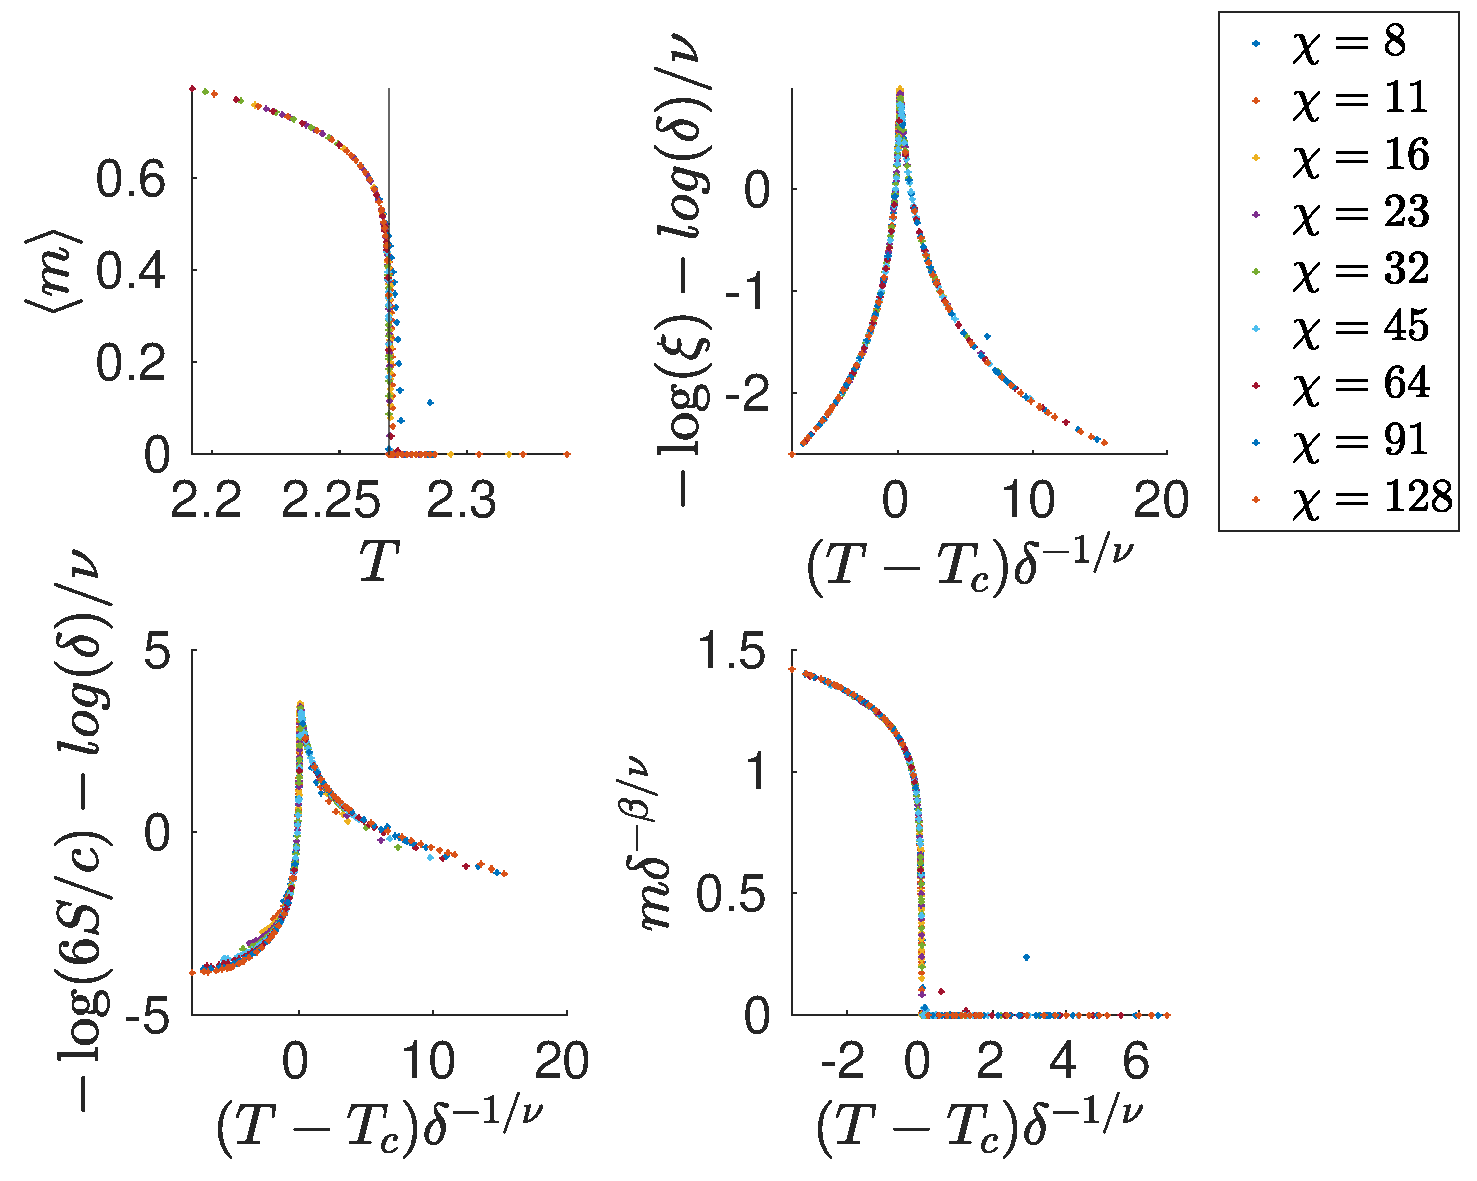
\includegraphics[height=\textheight]{../Figuren/phasediag/g0/zoomed_small.pdf}
        \end{figure}
    \end{minipage}
    \begin{minipage}{.24\textwidth}
        \begin{table}[]
            \begin{tabular}{l|l }
                      & $T_c$    \\
                \hline           \\
                Fit   & 2.691(9) \\
                Exact & 2.691853 \\

            \end{tabular}
        \end{table}
    \end{minipage}
\end{frame}
